%Arquivo contendo o capítulo Revisão Bibliográfica
\chapter{Revisão Bibliográfica} \label{cap:revbib}
Esse capítulo tem como objetivo descrever os principais conceitos apresentados para o desenvolvimento do \textit{software} proposto. Os conceitos envolvidos são: jogo pervasivo; gamificação; desenvolvimento multiplataforma; aplicativos de saúde e \textit{fitness}; avatares virtuais e geolocalização.

\section{Jogos Pervasivos}
Um jogo pervasivo é um tipo de jogo digital, no qual ao menos uma interação do usuário com o sistema transcorre no universo físico. Eles integram os aspectos físicos e sociais do mundo real em jogos digitais, estendendo a interação do jogador com o jogo, pois em ambientes virtuais a interface com o usuário está limitada ao uso dos periféricos do computador. Os recentes dispositivos celulares (\textit{smartphones}) e a popularização de tecnologias de rede sem fio 
(tais como, \textit{WiFi\footnote{WiFi é o termo popular para redes sem fio ethernet padrão  WLANs (Wireline Local Area Networks) \cite{lehr2003}.} e 3G\footnote{3G refere-se a terceira geração de serviços de dados móveis, fornecido por operadoras provedoras de redes móveis \cite{lehr2003}.}}) facilitam a extensão das interfaces homem-computador. \cite{magerkurth2005, vianna2013}. Um exemplo de jogo pervasivo é o Human Pacman. \par

\begin{figure}[h]
    \caption[Processo de coleta de um item no Human Pacman]{Processo de coleta de um item no Human Pacman \cite{cheok2003}.}
    \centerline{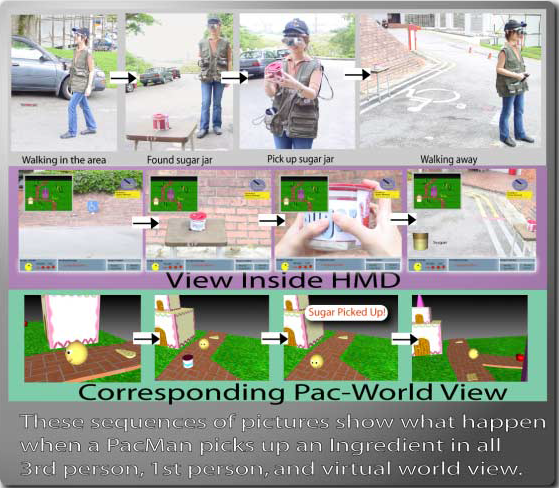
\includegraphics[width=20em]{figuras/humanpacman.png}}
    \label{fig:humanpacman}
\end{figure}

No Human Pacman, os jogadores interpretam o papel dos personagens do jogo Pac-Man no mundo real, enquanto vestem-se com trajes customizados integrados a dispositivos eletrônicos. Esses trajes permitem interação entre os jogadores via WiFi e interação com o sistema que insere elementos virtuais no mundo físico, através de técnicas de realidade aumentada, como ilustrado na figura \ref{fig:humanpacman} \cite{cheok2003}. 

\section{Gamificação}
A gamificação (do original em inglês \textit{gamification}) consiste na aplicação de mecanismos de jogos com o intuito de resolver problemas práticos ou motivar um público específico a realizar certas atividades em contextos fora de jogos. Alguns exemplos de aplicação de gamificação tem como objetivo: agilizar processos de aprendizagem ou treinamento; tornar mais agradáveis tarefas consideradas tediosas ou repetitivas; motivar usuários a reforçar a condição física e emocional e até usar jogos em forma de propagandas de produtos e serviços. O Duolingo\footnote{\url{https://www.duolingo.com/}} é um exemplo de \textit{software} "gamificado" para agilizar processos de aprendizagem de uma língua estrangeira e o SuperBetter\footnote{\url{https://www.superbetter.com/}}, para incentivar o usuário a reforçar o condicionamento físico. \cite{vianna2013, zichermann2011}.

\section{Desenvolvimento Multiplataforma}
Com a intenção de garantir que o \textit{software} possua portabilidade para plataformas \textit{mobile} e \textit{desktop} se fará uso do desenvolvimento \textit{Web}. Segundo \citet{lopes2013}, o desenvolvimento \textit{Web} é democrático, aberto e acessível, pois praticamente, todo dispositivos possui um navegador (\textit{web browser}). Uma aplicação \textit{Web} garante acesso a um número maior de usuários do que uma aplicação nativa para um determinado dispositivo. Lopes também salienta que é cada vez mais comum usar as linguagens fundamentais da \textit{Web} para desenvolver aplicativos \textit{mobile}. A subseção seguinte versará sobre as tecnologias fundamentais do desenvolvimento \textit{Web}.

\subsection{Lado do Cliente}
As tecnologias fundamentais usadas em sistemas \textit{Web}, no lado do cliente, são o HTML (\textit{Hyper Text Markup Language}), o CSS (\textit{Cascading Style Sheets}) e o JavaScript (JS). \par

HTML5 é a versão atual do HTML, linguagem de marcação para escrever a estrutura principal de páginas \textit{Web}. HTML fornece instruções aos \textit{web browsers} (exemplos: Chrome, IE, Firefox) sobre o que exibir em uma página. Cada conteúdo é representado por um conjunto de elementos pré-definidos chamados \textit{tags} \cite{html5}. \par 

CSS é a linguagem usada para definir o estilo e o \textit{layout} do conteúdo de uma página HTML. Ela também permite ajustar o \textit{layout} das aplicações para qualquer tamanho de tela, inclusive o \textit{mobile}. Esta característica é importante para o \textit{software} desde trabalho, o qual pretende ser multiplataforma. A versão atual do CSS é o CSS3 \cite{css3}. \par
 
JS é uma linguagem de programação interpretada e orientada a objetos, usada para manipular o comportamento de páginas HTML. Possui recursos para alterar o conteúdo das páginas, o estilo delas e validar entradas do usuário. \cite{javascript}. \par

No desenvolvimento do lado do cliente também podem ser empregados \textit{frameworks} e bibliotecas. Estes se propõem a facilitar o uso das linguagens listadas anteriormente, assegurar questões de compatibilidade entre navegadores, assegurar questões de segurança e confiabilidade e de portabilidade para diferentes dispositivos. \par

Os seguintes \textit{frameworks} serão investigados para o possível uso no desenvolvimento do \textit{software} deste trabalho: Bootstrap\footnote{\url{http://getbootstrap.com/}}, para desenvolvimento de páginas \textit{Web} responsivas e adaptáveis para dispositivos com tamanhos diversos; AngularJS\footnote{\url{https://angularjs.org/}}, usado para tornar páginas HTML estáticas em páginas dinâmicas, estendendo o vocabulário do HTML; e jQuery\footnote{\url{https://jquery.com/}}, usado para facilitar e estender o JS. \par
 
A plataforma Cordova\footnote{\url{https://cordova.apache.org/}}, para conversão de sistemas \textit{Web} em aplicações nativas \textit{mobile}, também será investigada. Ela permite atribuir ao \textit{software} acesso aos recursos de \textit{hardware} dos dispositivos \textit{mobile}.

\subsection{Lado do Servidor} \label{sec:server}
Atualmente o pódio das tecnologias para o desenvolvimento \textit{Web} do lado do Servidor está ocupado pelo PHP, em primeiro lugar; ASP.NET em segundo e o Java, em terceiro \cite{w3techs2015}. \par

Java \textit{Web} consiste na implementação das APIs de Servlets e JavaServer Pages (JSP). Servlet é a tecnologia usada pelo Java para geração de páginas HTML dinâmicas, são classes Java com HTML embutido. Páginas JSP consistem no inverso, são estruturadas como páginas HTML com código Java embutido. Servlets e JSP podem ser desenvolvidos na plataforma Java Enterprise Edition (Java EE). A Java EE consiste em um conjunto de especificações para várias APIs de desenvolvimento Java para \textit{Web} \cite{basham2008}. Os pontos fortes do Java \textit{Web} estão na portabilidade para diferentes plataformas de \textit{hardware}, banco de dados e servidores e a grande quantidade de \textit{frameworks} existentes, tais como Primefaces\footnote{\url{http://www.primefaces.org/}} e Spring\footnote{\url{http://spring.io/}}. \par

ASP.NET é uma tecnologia da Microsoft, parte do .NET \textit{Framework} para desenvolvimento de aplicações \textit{Web}. O desenvolvimento com ASP.NET pode ser feito com qualquer linguagem compatível com o .NET. Algumas das vantagens desta tecnologia envolvem a separação clara entre a interface do usuário e a lógica de programação; a familiaridade com o desenvolvimento \textit{desktop}; a ferramenta de desenvolvimento Visual Studio, com diversos recursos para facilitar o trabalho do desenvolvedor e a integração com todos os recursos do \textit{framework} .NET \cite{imar2014}. As desvantagens do ASP.NET são: sua limitação ao sistema operacional Windows e a licença de uso do Visual Studio não ser gratuita. \par

PHP é uma linguagem de programação presente em 10 milhões de sites no mundo inteiro. O PHP adiciona dinamismo às páginas estáticas e automatiza tarefas, diminuindo mão-de-obra. Possui portabilidade para várias plataformas \textit{desktop} (exemplos: Linux, Unix e Windows); possui código aberto e licença de uso gratuita; suporta vários bancos de dados (entre eles: MySQL, Oracle e PostgreSQL). Sua versão mais recente é o PHP 5 \cite{niederauer2004, welling2003}. \par

Outros pontos fortes do PHP envolvem sua alta performance (um único servidor pode lidar com milhões de acessos por dia); bibliotecas nativas para várias tarefas comuns na \textit{Web} (funções para gerenciamento de imagens, conexão com \textit{web services}, interpretação de XML, envio de \textit{email}, gerenciamento de \textit{cookies} e geração de documentos PDF); fácil aprendizado (a sintaxe de PHP é baseada em outras linguagens, entre elas, C e Perl); suporte ao desenvolvimento orientado a objetos e disponibilidade de suporte técnico \cite{welling2003}. \par

Pretende-se usar a linguagem PHP para desenvolvimento do lado do servidor, pois comparado com as outras duas principais linguagens (ASP.NET e Java) o PHP se destaca por sua licença gratuita, portabilidade e suporte nativo (sem \textit{frameworks}) a funcionalidades que serão essenciais no software deste trabalho, tais como: gerenciamento de imagens, interpretação de arquivos JSON e acesso a banco de dados. \par

No quesito sistemas de gerenciamento de banco de dados (SGDB), os três mais usados atualmente segundo o \textit{site} da DB-Engines são o Oracle em primeiro lugar, o MySQL em segundo e o Microsoft SQL Server em terceiro. O MySQL possui licença de uso \textit{open source} e versão gratuita sem restrições, enquanto o Oracle e o Microsoft SQL Server são \textit{softwares} com licença de uso comercial, por estes motivos pretende-se fazer uso dele. \par

\section{Aplicativos de Saúde e \textit{Fitness}}
Aplicativos de Saúde e \textit{Fitness} são \textit{softwares} desenvolvidos para dispositivos \textit{mobile} com o objetivo de estimular o usuário a praticar atividades benéficas à saúde e ao bem-estar \cite{bonome2012}. Alguns exemplos dessa categoria de aplicativos são o Strava\footnote{\url{https://www.strava.com/}} e o  Runtastic\footnote{\url{https://www.runtastic.com/}}. \par

\section{Avatares Virtuais}
Avatares são corpos virtuais criados para representar a identidade e ações de um usuário em um mundo virtual. Eles são usados como ferramentas de comunicação e para representar visualmente os usuários. Uma das principais características dos avatares é a sua customização, orientada pelo desejo de quem o cria \cite{ducheneaut2009}. Um exemplo de aplicativo específico para criação de avatares e utilização destes como ferramente de socialização entre os usuários é o \textit{BuddyPoke}, ver figura \ref{fig:avatar}. \par

\begin{figure}[hb]
    \caption{Exemplo de avatar criado no aplicativo BuddyPoke.}
    \centerline{
\includegraphics[width=17em]{figuras/avatar.png}}
    \label{fig:avatar}
\end{figure}
\centerline{Fonte: Página oficial do BuddyPoke na \textit{Web}\footnote{Disponível em: <\url{http://www.buddypoke.com/}>. Acesso em jun. 2015.}}

\section{Geolocalização}
Geolocalização é o termo usado para descrever o posicionamento geográfico de um objeto no planeta, a partir de seus valores de latitude e longitude \cite{aires2014}. Essas coordenadas são obtidas utilizando \textit{Global Positioning System} (GPS), um sistema desenvolvido e mantido pelas Forças Aéreas dos Estados Unidos. Este sistema consiste em três segmentos: o espacial, composto por 24 satélites operantes em órbita e transmitindo sinais de radio; o controle, o qual consiste nas estações de controle que mantêm os satélites funcionando adequadamente; e o segmento do usuário, o qual compreende os aparelhos receptores dos sinais vindos dos satélites \cite{gpsgov}. O funcionamento do GPS é ilustrado na figura \ref{fig:gps}. \par

\begin{figure}[h]
    \caption[Funcionamento do GPS]{Funcionamento do GPS \cite{cesani2013}.}
    \centerline{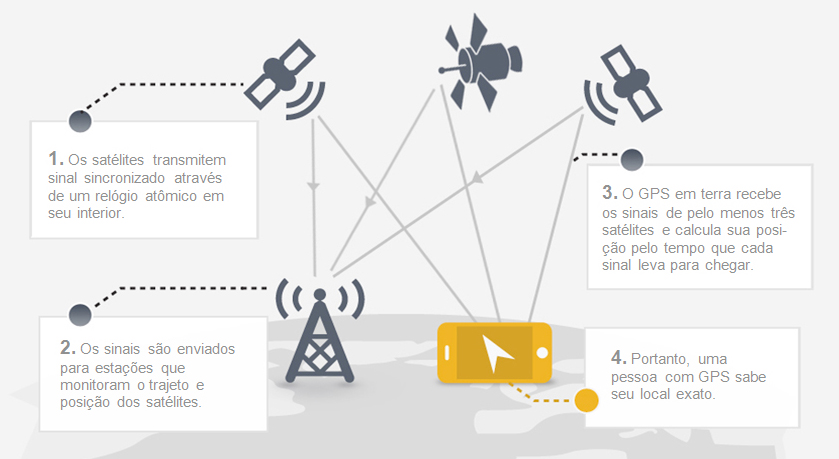
\includegraphics[width=30em]{figuras/gps.png}}
    \label{fig:gps}
\end{figure}

No entanto, o uso de GPS tem suas limitações. Segundo \citet{sukaphat2013}, os sinais de GPS possuem um alcance limitado e uma capacidade baixa de atravessar barreiras. Estas características impedem o funcionamento adequado desta tecnologia em ambientes fechados. \par

%\section{Conclusões}
%Reunir as ideias principais abordadas no capítulo.